\chapter{Specifikacija programske potpore}
		
	\section{Funkcionalni zahtjevi}
			
			\noindent \textbf{Dionici:}
			
			\begin{packed_enum}
				
				\item Voditelji
				\item Natjecatelji				
				\item Administrator
				\item Razvojni tim
				
			\end{packed_enum}
			
			\noindent \textbf{Aktori i njihovi funkcionalni zahtjevi:}
			
			
			\begin{packed_enum}
				\item  \underbar{Neregistrirani/neprijavljeni korisnik (inicijator) može:}
				
				\begin{packed_enum}
					
					\item vidjeti kalendar s budućim natjecanjima
					\item pregledati dostupne zadatke na stranici
					\item pregledati profile natjecatelja i voditelja
					\item registrirati se u sustav stvaranjem novog korisničkog računa pri čemu odabire jednu od uloga (natjecatelj ili voditelj), a potrebni su mu: korisničko ime, fotografija, lozinka, ime, prezime te email adresa
					
				\end{packed_enum}
			
				\item  \underbar{Natjecatelj (inicijator) može:}
				
				\begin{packed_enum}
					
					\item sudjelovati na natjecanju
					\item vidjeti rang listu natjecatelja na natjecanju kojeg je i sam bio sudionik
					\item vidjeti popis svih učitanih rješenja od ostalih sudionika za prethodno završena natjecanja
					\item pristupiti rješavanju već objavljenih zadataka
					\item izraditi virtualno natjecanje odabirom nekog prošlog natjecanja ili nasumičnim generiranjem zadataka 
					\item vidjeti vlastiti profil s osobnim podacima, statistikom o broju točno riješenih zadatka, broju isprobanih zadataka te prikaz pehara za osvojena natjecanja
					
				\end{packed_enum}
				
				\item  \underbar{Aktivni natjecatelj (inicijator) može:}
				
				\begin{packed_enum}
					
					\item rješavati zadatke i slati datoteke s programskim kodom tijekom natjecanja na kojem se natječe 
					\item osvojiti bodove na natjecanju s obzirom na potrošeno vrijeme za rješavanje zadatka i postotak točnih primjera 
					\item na temelju postignuća za prva tri mjesta osvojiti pehar koji je vidljiv na vlastitom profilu
					
				\end{packed_enum}
				
				\item  \underbar{Voditelj (inicijator) može:}
				
				\begin{packed_enum}
					
					\item pregledati dostupne zadatke na stranici
					\item izraditi novi zadatak pri čemu treba definirati: naziv zadatka, broj bodova, vremensko ograničenje, tekst zadatka i primjere za evaluaciju
					\item organizirati novo natjecanje pri čemu treba definirati: vrijeme početka i završetka, broj zadataka, koji zadaci će biti aktivni te po želji sličicu pehara
					\item uređivati vlastite prethodno objavljene zadatke te natjecanja
					\item vidjeti vlastiti profil s osobnim podacima, popisom učitanih zadataka s mogućnošću sortiranja te kalendar s popisom objavljenih natjecanja
										
				\end{packed_enum}
				
				\item  \underbar{Administrator (inicijator) može:}
				
				\begin{packed_enum}
					
					\item uređivati sve zadatke i natjecanja
					\item potvrditi voditelja prilikom registracije
					\item vidjeti popis svih registriranih korisnika i njihovih osobnih podataka
					\item mijenjati dodijeljena prava i osobne podatke

				\end{packed_enum}
				
				\item  \underbar{Baza podataka (sudionik) može:}
				
				\begin{packed_enum}
					
					\item pohranjuje sve podatke o korisnicima i njihovim ovlastima te zadacima i natjecanjima
					\item pohranjuje rezultate natjecanja, rješenja zadataka i statistiku natjecatelja			
					
				\end{packed_enum}
			\end{packed_enum}
			
			\eject 
			
			
				
			\subsection{Obrasci uporabe}
				
				\textbf{\textit{dio 1. revizije}}
				
				\subsubsection{Opis obrazaca uporabe}
					\textit{Funkcionalne zahtjeve razraditi u obliku obrazaca uporabe. Svaki obrazac je potrebno razraditi prema donjem predlošku. Ukoliko u nekom koraku može doći do odstupanja, potrebno je to odstupanje opisati i po mogućnosti ponuditi rješenje kojim bi se tijek obrasca vratio na osnovni tijek.}\\
					

%					\noindent \underbar{\textbf{UC$<$broj obrasca$>$ -$<$ime obrasca$>$}}
%					\begin{packed_item}
%	
%						\item \textbf{Glavni sudionik: }$<$sudionik$>$
%						\item  \textbf{Cilj:} $<$cilj$>$
%						\item  \textbf{Sudionici:} $<$sudionici$>$
%						\item  \textbf{Preduvjet:} $<$preduvjet$>$
%						\item  \textbf{Opis osnovnog tijeka:}
%						
%						\item[] \begin{packed_enum}
%	
%							\item $<$opis korak jedan$>$
%							\item $<$opis korak dva$>$
%							\item $<$opis korak tri$>$
%							\item $<$opis korak četiri$>$
%							\item $<$opis korak pet$>$
%						\end{packed_enum}
%						
%						\item  \textbf{Opis mogućih odstupanja:}
%						
%						\item[] \begin{packed_item}
%	
%							\item[2.a] $<$opis mogućeg scenarija odstupanja u koraku 2$>$
%							\item[] \begin{packed_enum}
%								
%								\item $<$opis rješenja mogućeg scenarija korak 1$>$
%								\item $<$opis rješenja mogućeg scenarija korak 2$>$
%								
%							\end{packed_enum}
%							\item[2.b] $<$opis mogućeg scenarija odstupanja u koraku 2$>$
%							\item[3.a] $<$opis mogućeg scenarija odstupanja  u koraku 3$>$
%							
%						\end{packed_item}
%					\end{packed_item}
					
					\noindent \underbar{\textbf{UC1 - Pregled kalendara}}
					\begin{packed_item}
						
						\item \textbf{Glavni sudionik: } Korisnik
						\item \textbf{Cilj:} Pregledati kalendar s nadolazećim natjecanjima 
						\item \textbf{Sudionici:} baza podataka
						\item \textbf{Preduvjet:} -
						\item \textbf{Opis osnovnog tijeka:}
						
						\item[] \begin{packed_enum}
							\item Korisnik otvara početnu stranicu web aplikacije
							\item Prikazuje se kalendar
							\item Korisnik odabire određeni datum
							\item Aplikacija prikazuje popis nadolazećih natjecanja za odabrani datum
							\item Korisnik odabire natjecanje
							\item Prikazuju se detalji i informacije o odabranom natjecanju
						\end{packed_enum}
					\end{packed_item}
					
					
					\noindent \underbar{\textbf{UC2 - Pregled zadataka}}
					\begin{packed_item}
						
						\item \textbf{Glavni sudionik: }Korisnik
						\item \textbf{Cilj:} Pregledati zadatke završenih natjecanja
						\item \textbf{Sudionici:} baza podataka
						\item \textbf{Preduvjet:} -
						\item \textbf{Opis osnovnog tijeka:}
						
						\item[] \begin{packed_enum}
							\item Korisnik odabire završeno natjecanja
							\item Prikazuje se lista zadatka povezana s odabranim natjecanjem
							\item Korisnik odabire specifičan zadatak
							\item Aplikacija prikazuje detalje zadatka
						\end{packed_enum}
					\end{packed_item}
					
					
					\noindent \underbar{\textbf{UC3 - Pregled profila natjecatelja i voditelja}}
					\begin{packed_item}
						
						\item \textbf{Glavni sudionik: }Korisnik
						\item \textbf{Cilj:} Pregledati profile natjecatelja i voditelja
						\item \textbf{Sudionici:} baza podataka
						\item \textbf{Preduvjet:} -
						\item \textbf{Opis osnovnog tijeka:}
						
						\item[] \begin{packed_enum}
							\item Korisnik otvara profil određenog korisnika klikom na njihovo korisničko ime
							\item Ako je otvoren profil natjecatelja, aplikacija prikazuje informacije o broju točno riješenih zadataka, broju isprobanih zadataka te osvojene pehare
							\item Ako je otvoren profil voditelja, aplikacija prikazuje popis učitanih zadataka i kalendar s popisom objavljenih natjecanja
						\end{packed_enum}
					\end{packed_item}
					
					
					
					\noindent \underbar{\textbf{UC4 - Registracija}}
					\begin{packed_item}
						
						\item \textbf{Glavni sudionik: }Korisnik
						\item  \textbf{Cilj:} Stvoriti korisnički račun
						\item  \textbf{Sudionici:} baza podataka, administrator 
						\item  \textbf{Preduvjet:} korisnik nije prethodno registriran ili prijavljen u sustav
						\item  \textbf{Opis osnovnog tijeka:}
						
						\item[] \begin{packed_enum}
							
							\item Korisnik odabire opciju za registraciju 
							\item Korisnik popunjava obrazac za registraciju s potrebnim podacima 
							\item Korisnik na svoju e-mail adresu prima obavijest i zahtjev za potvrdu registracije
							\item Ako je korisnik odabrao ulogu "voditelj", sustav dodatno šalje obavijest administratoru 
							\item Administrator potvrđuje registraciju voditelja 
						\end{packed_enum}
						
						\item  \textbf{Opis mogućih odstupanja:}
						\item[] \begin{packed_item}
							
							\item[2.a] Već zauzeto korisničko ime ili e-mail adresa, uneseni podaci u nedozvoljenom formatu ili neispravna e-mail adresa 
							\item[] \begin{packed_enum}
								
								\item Sustav obavještava korisnika o neuspjelom unosu i prikazuje relevantne poruke o greškama 
								\item Korisnik mijenja potrebne podatke te završava unos ili odustaje od registracije 
								
							\end{packed_enum}
							
							\item[5.a] Administrator odbija zahtjev za registraciju voditelja natjecanja:
							\item[] \begin{packed_enum}
								
								\item Sustav obavještava korisnika putem e-maila
								
							\end{packed_enum}
						\end{packed_item}
					\end{packed_item}
					
					\noindent \underbar{\textbf{UC5 - Prijava}}
					\begin{packed_item}
						
						\item \textbf{Glavni sudionik: }Korisnik
						\item \textbf{Cilj:} Dobiti pristup korisničkom sučelju
						\item \textbf{Sudionici:} baza podataka
						\item \textbf{Preduvjet:} korisnik je registriran u sustav, ali nije prijavljen
						\item \textbf{Opis osnovnog tijeka:}
						\item[] \begin{packed_enum}
							\item Korisnik unosi korisničko ime i lozinku
							\item Sustav potvrđuje ispravnosti unesenih podataka
							\item Korisniku je omogućen pristup korisničkim funkcijama
						\end{packed_enum}
						
						\item  \textbf{Opis mogućih odstupanja:}
						
						\item[] \begin{packed_item}
							
							\item[2.a] Neispravno korisničko ime/lozinka
							\item[] \begin{packed_enum}
								
								\item Sustav obavještava korisnika o neuspjelom upisu i vraća ga na stranicu za registraciju
								
							\end{packed_enum}
						\end{packed_item}
					\end{packed_item}
					
					\noindent \underbar{\textbf{UC6 - Pregled profila}}
					\begin{packed_item}
						
						\item \textbf{Glavni sudionik: }Korisnik
						\item \textbf{Cilj:} Pregledati vlastiti profil
						\item \textbf{Sudionici:} baza podataka
						\item \textbf{Preduvjet:} korisnik je prijavljen
						\item \textbf{Opis osnovnog tijeka:}
						\item[] \begin{packed_enum}
							\item Korisnik pristupa opciji "Moj profil" klikom na ikonu profila
							\item Aplikacija prikazuje podatke o korisniku (ime, fotografija, lozinka, ime, prezime i e-mail adresa)
						\end{packed_enum}
					\end{packed_item}
					
					
					
					\noindent \underbar{\textbf{UC7 - Pregled vlastite statistike}}
					\begin{packed_item}
						
						\item \textbf{Glavni sudionik: }Korisnik (natjecatelj)
						\item \textbf{Cilj:} Pregledati vlastitu statistiku unutar web aplikacije
						\item \textbf{Sudionici:} baza podataka
						\item \textbf{Preduvjet:} korisnik je prijavljen
						\item \textbf{Opis osnovnog tijeka:}
						
						\item[] \begin{packed_enum}
							\item Korisnik pristupa svojem profilu i odabire opciju "Moje statistike"
							\item Aplikacija prikazuje statistike korisnika(broj točno riješenih zadataka, broj isprobanih zadataka, pehare za osvojena natjecanja)
						\end{packed_enum}
					\end{packed_item}

					
					\noindent \underbar{\textbf{UC8 - Pregled vlastitih zadataka}}
					\begin{packed_item}
						
						\item \textbf{Glavni sudionik: }Korisnik (voditelj)
						\item \textbf{Cilj:} Pregledati popis svih vlastito objavljenih zadataka
						\item \textbf{Sudionici:} baza podataka
						\item \textbf{Preduvjet:} korisnik je prijavljen
						\item \textbf{Opis osnovnog tijeka:}
						
						\item[] \begin{packed_enum}
							\item Voditelj odabire opciju za prikaz vlastitih zadataka
							\item Prikazuju se svi objavljeni zadaci tog voditelja
						\end{packed_enum}
					\end{packed_item}
										
										
										
					\noindent \underbar{\textbf{UC9 – Sudjelovanje na natjecanju}}
					\begin{packed_item}
						
						\item \textbf{Glavni sudionik: }Korisnik (natjecatelj)
						\item \textbf{Cilj:} Pristupiti natjecanju 
						\item \textbf{Sudionici:} baza podataka
						\item \textbf{Preduvjet:} korisnik je prijavljen i postoji natjecanje u tijeku
						\item \textbf{Opis osnovnog tijeka:}
						
						\item[] \begin{packed_enum}
							\item Prikazuju se informacije o natjecanju u tijeku i natjecatelj potvrđuje da želi sudjelovati na natjecanju 
							\item Natjecatelju se prikazuju zadaci koji su dio natjecanja te preostalo vrijeme do kraja natjecanja
						\end{packed_enum}
					\end{packed_item}
								
					
					
					\noindent \underbar{\textbf{UC10 – Prijenos datoteke rješenja}}
					\begin{packed_item}
						
						\item \textbf{Glavni sudionik: }Korisnik (natjecatelj, aktivni natjecatelj)
						\item \textbf{Cilj:} Prenijeti datoteku kao rješenje nekog zadatka na natjecanju
						\item \textbf{Sudionici:} baza podataka
						\item \textbf{Preduvjet:} natjecatelj je pristupio natjecanju ili rješavanju zadataka
						\item \textbf{Opis osnovnog tijeka:}
						
						\item[] \begin{packed_enum}
							\item Korisnik nakon napisanog rješenja zadatka odabire opciju za predaju rješenja
							\item Korisnik odabire datoteku s rješenjem koju želi predati i potvrđuje odabir
							\item Datoteka se prenosi, predaje kao rješenje i šalje na evaluaciju
						\end{packed_enum}
						
							\item  \textbf{Opis mogućih odstupanja:}
							
							\item[] \begin{packed_item}
								
								\item[2.a] Odabir pogrešne datoteke
								\item[] \begin{packed_enum}
									
									\item Aktivni natjecatelj odabire opciju za brisanje datoteke 
									\item Aktivni natjecatelj ponovno kreće s 1. korakom iz osnovnog tijeka
																
								\end{packed_enum}
							\end{packed_item}
						\end{packed_item}
									
									
					
					\noindent \underbar{\textbf{UC11 – Pregled rang liste}}
					\begin{packed_item}
						
						\item \textbf{Glavni sudionik: }Korisnik (natjecatelj)
						\item \textbf{Cilj:} Pregledati rang listu nekog natjecanja
						\item \textbf{Sudionici:} baza podataka
						\item \textbf{Preduvjet:} korisnik je prijavljen kao natjecatelj
						\item \textbf{Opis osnovnog tijeka:}
						
						\item[] \begin{packed_enum}
							\item Natjecatelj odabire opciju za prikaz prošlih natjecanja na kojima je sudjelovao
							\item Odabire natjecanje za koje želi vidjeti rang listu ostalih sudionika i odabire prikaz rang liste
							\item Otvara se popis s prikazom postignuća ostalih sudionika po broju ostvarenih bodova
						\end{packed_enum}
					\end{packed_item}
										
										
					\noindent \underbar{\textbf{UC12 – Pregled rješenja zadataka}}
					\begin{packed_item}
						
						\item \textbf{Glavni sudionik: }Korisnik (natjecatelj)
						\item \textbf{Cilj:} Vidjeti tuđa rješenja zadataka s nekog natjecanja
						\item \textbf{Sudionici:} Baza podataka
						\item \textbf{Preduvjet:} Natjecatelj je sudjelovao na natjecanju koje je završilo
						\item \textbf{Opis osnovnog tijeka:}
						
						\item[] \begin{packed_enum}
							\item Natjecatelj odabire opciju za prikaz prošlih natjecanja na kojima je sudjelovao
							\item Natjecatelj odabire natjecanje za koje želi vidjeti predana rješenja 
							\item Prikazuju se informacije o natjecanju s popisom svih predanih rješenja
							\item Odabirom opcije za prikaz natjecanja po zadacima prikazuje se pregled zadataka s tog natjecanja
							\item Odabirom zadatka otvara se tekst zadatka s prikazom svih predanih rješenja drugih sudionika uz informacije o uspješnosti predanog rješenja
						\end{packed_enum}
					\end{packed_item}
										
										
										
					\noindent \underbar{\textbf{UC13 – Rješavanje zadataka}}
					\begin{packed_item}
						
						\item \textbf{Glavni sudionik: }Korisnik (natjecatelj)
						\item \textbf{Cilj:} Vježbanje već objavljenih zadataka
						\item \textbf{Sudionici:} baza podataka
						\item \textbf{Preduvjet:} korisnik je prijavljen kao natjecatelj
						\item \textbf{Opis osnovnog tijeka:}
						
						\item[] \begin{packed_enum}
							\item Natjecatelj odabire opciju za prikaz svih objavljenih zadataka
							\item Prikazuje se popis svih zadataka
							\item Odabirom zadatka koji želi rješavati otvara se sučelje slično onom na natjecanju koje natjecatelju omogućuje učitavanje datoteke kao rješenja zadataka i evaluiranje istog
						\end{packed_enum}
					\end{packed_item}
									
								
					
					\noindent \underbar{\textbf{UC14 – Izrada virtualnog natjecanja}}
					\begin{packed_item}
						
						\item \textbf{Glavni sudionik: }Korisnik (natjecatelj)
						\item \textbf{Cilj:} Vježbanje simuliranjem pravog natjecanja
						\item \textbf{Sudionici:} baza podataka
						\item \textbf{Preduvjet:} postoji barem jedno završeno natjecanje i/ili barem jedan javno vidljiv zadatak u bazi
						\item \textbf{Opis osnovnog tijeka:}
						
						\item[] \begin{packed_enum}
							\item Natjecatelj odabire opciju “virtualno natjecanje”
							\item Otvara se prikaz s dvije mogućnosti odabira
							\item Natjecatelj odabire jednu od dvije opcije - stvaranje natjecanja pokretanjem nekog prošlog natjecanja iz kalendara ili stvaranje natjecanja nasumičnim odabirom zadataka iz baze zadataka
							\item Natjecanje se stvara i natjecatelj može krenuti s rješavanjem zadataka
						\end{packed_enum}
					\end{packed_item}
										
										
										
					\noindent \underbar{\textbf{UC15 – Unos novog zadatka}}
					\begin{packed_item}
						
						\item \textbf{Glavni sudionik: }Korisnik (voditelj)
						\item \textbf{Cilj:} Stvoriti novi zadatak u bazi postojećih zadataka
						\item \textbf{Sudionici:} baza podataka
						\item \textbf{Preduvjet:} korisnik je prijavljen kao voditelj
						\item \textbf{Opis osnovnog tijeka:}
						
						\item[] \begin{packed_enum}
							\item Voditelj odabire opciju za unos novog zadatka
							\item Otvara se forma gdje voditelj upisuje naziv zadatka, broj bodova koji nosi, vremensko ograničenje izvršavanja, tekst zadatka i primjere za evaluaciju
							\item Voditelj odabire želi li zadatak stvoriti kao privatan ili javan
							\item Voditelj potvrđuje unos zadatka
							\item Zadatak se pohranjuje u bazu ostalih zadataka s informacijom o autoru zadatka
						\end{packed_enum}
						
						\item  \textbf{Opis mogućih odstupanja:}
						\item[] \begin{packed_item}
							
							\item[2.a] Voditelj ostavlja prazno neko polje u formi i pokušava predati takav zadatak
							\item[] \begin{packed_enum}
								
								\item Sustav ga obavještava o neispravnom pokušaju predaje zadatka 
								\item Sustav omogućuje ponovno ispunjavanje forme u svrhu ispravne predaje
								
							\end{packed_enum}
						\end{packed_item}
					\end{packed_item}
					
					\noindent \underbar{\textbf{UC16 – Uređivanje zadatka}}
					\begin{packed_item}
						
						\item \textbf{Glavni sudionik: }Korisnik (voditelj)
						\item \textbf{Cilj:} Uređivanje postojećeg zadatka
						\item \textbf{Sudionici:} baza podataka
						\item \textbf{Preduvjet:} postoji zadatak koji je prijavljeni voditelj unio u bazu
						\item \textbf{Opis osnovnog tijeka:}
						
						\item[] \begin{packed_enum}
							\item Voditelj odabire opciju “moji zadaci”
							\item Otvara se pregled svih zadataka koje je voditelj unio u sustav
							\item Voditelj odabire opciju uređivanja zadataka
							\item Otvara se forma slična onoj kod unosa novog zadatka koja voditelju omogućuje izmjenu podataka te spremanje istih
						\end{packed_enum}
					\end{packed_item}
					
					
					
					\noindent \underbar{\textbf{UC17 – Organiziranje natjecanja}}
					\begin{packed_item}
						
						\item \textbf{Glavni sudionik: }Korisnik (voditelj)
						\item \textbf{Cilj:} Organizirati novo natjecanje
						\item \textbf{Sudionici:} baza podataka
						\item \textbf{Preduvjet:} korisnik je prijavljen
						\item \textbf{Opis osnovnog tijeka:}
						
						\item[] \begin{packed_enum}
							\item Voditelj odabire opciju za organiziranje novog natjecanja
							\item Otvara se forma gdje voditelj odabire vrijeme početka i završetka natjecanja, broj zadataka, koji zadaci će biti aktivni te po želji učitava sličicu pehara
							\item Voditelj potvrđuje podatke o novom natjecanju
							\item Natjecanje se dodaje u kalendar natjecanja
							
						\end{packed_enum}
						
						\item  \textbf{Opis mogućih odstupanja:}
						\item[] \begin{packed_item}
							
							\item[2.a] Voditelj ne ispunjava neko polje u formi i pokušava potvrditi natjecanje
							\item[] \begin{packed_enum}
								
								\item Sustav ga obavještava o neispravnosti ispunjene forme
								\item Sustav omogućuje ponovno ispunjavanje forme u svrhu ispravne predaje
								
							\end{packed_enum}
						\end{packed_item}
					\end{packed_item}
										
					\noindent \underbar{\textbf{UC18 – Uređivanje natjecanja}}
					\begin{packed_item}
						
						\item \textbf{Glavni sudionik: }Korisnik (voditelj)
						\item \textbf{Cilj:} Uređivanje postojećeg natjecanja
						\item \textbf{Sudionici:} baza podataka
						\item \textbf{Preduvjet:} postoji natjecanje koje je prijavljeni voditelj organizirao, a ono nije u tijeku ili završeno
						\item \textbf{Opis osnovnog tijeka:}
						
						\item[] \begin{packed_enum}
							\item Voditelj odabire opciju “moja natjecanja”
							\item Otvara se pregled svih natjecanja koje je voditelj organizirao
							\item Voditelj odabire opciju uređivanja natjecanja kojemu želi izmijeniti podatke
							\item Otvara se pregled sličan onom prilikom organiziranja novog natjecanja koji voditelju omogućuje izmjenu i spremanje novih postavki natjecanja
						\end{packed_enum}
					\end{packed_item}
					
					\noindent \underbar{\textbf{UC19 – Pregled svih korisnika u bazi}}
					\begin{packed_item}
						
						\item \textbf{Glavni sudionik: }Administrator
						\item \textbf{Cilj:} Pregled svih registriranih korisnika u bazi
						\item \textbf{Sudionici:} baza podataka
						\item \textbf{Preduvjet:} -
						\item \textbf{Opis osnovnog tijeka:}
						
						\item[] \begin{packed_enum}
							\item Administrator odabire opciju prikaza korisnika u bazi
							\item Otvara se popis svih registriranih BytePit korisnika
							
						\end{packed_enum}
					\end{packed_item}
					
					
					
					\noindent \underbar{\textbf{UC20 – Izmjena osobnih podataka}}
					\begin{packed_item}
						
						\item \textbf{Glavni sudionik: }Administrator
						\item \textbf{Cilj:} Uređivanje podataka nekog korisnika
						\item \textbf{Sudionici:} baza podataka
						\item \textbf{Preduvjet:} postoji barem jedan registrirani korisnik u bazi 
						\item \textbf{Opis osnovnog tijeka:}
						
						\item[] \begin{packed_enum}
							\item Administrator odabire opciju prikaza korisnika u bazi
							\item Otvara se popis svih registriranih BytePit korisnika
							\item Odabirom korisnika prikazuju se njegovi osobni podaci s mogućnošću izmjene istih uključujući i izmjenu dodijeljene uloge korisniku
							
						\end{packed_enum}
					\end{packed_item}
					
					
					\noindent \underbar{\textbf{UC21 – Brisanje korisnika}}
					\begin{packed_item}
						
						\item \textbf{Glavni sudionik: }Administrator
						\item \textbf{Cilj:} Brisanje postojećeg korisnika iz baze podataka
						\item \textbf{Sudionici:} baza podataka
						\item \textbf{Preduvjet:} postoji barem jedan registrirani korisnik u bazi
						\item \textbf{Opis osnovnog tijeka:}
						
						\item[] \begin{packed_enum}
							\item Administrator odabire opciju prikaza korisnika u bazi
							\item Otvara se popis svih registriranih BytePit korisnika
							\item Administrator odabire i potvrđuje opciju brisanja korisnika 
							\item Korisnik se briše iz baze podataka
							
						\end{packed_enum}
					\end{packed_item}
					
				
					
				\subsubsection{Dijagrami obrazaca uporabe}
					
					\textit{Prikazati odnos aktora i obrazaca uporabe odgovarajućim UML dijagramom. Nije nužno nacrtati sve na jednom dijagramu. Modelirati po razinama apstrakcije i skupovima srodnih funkcionalnosti.}
					
					\begin{figure}[H]
						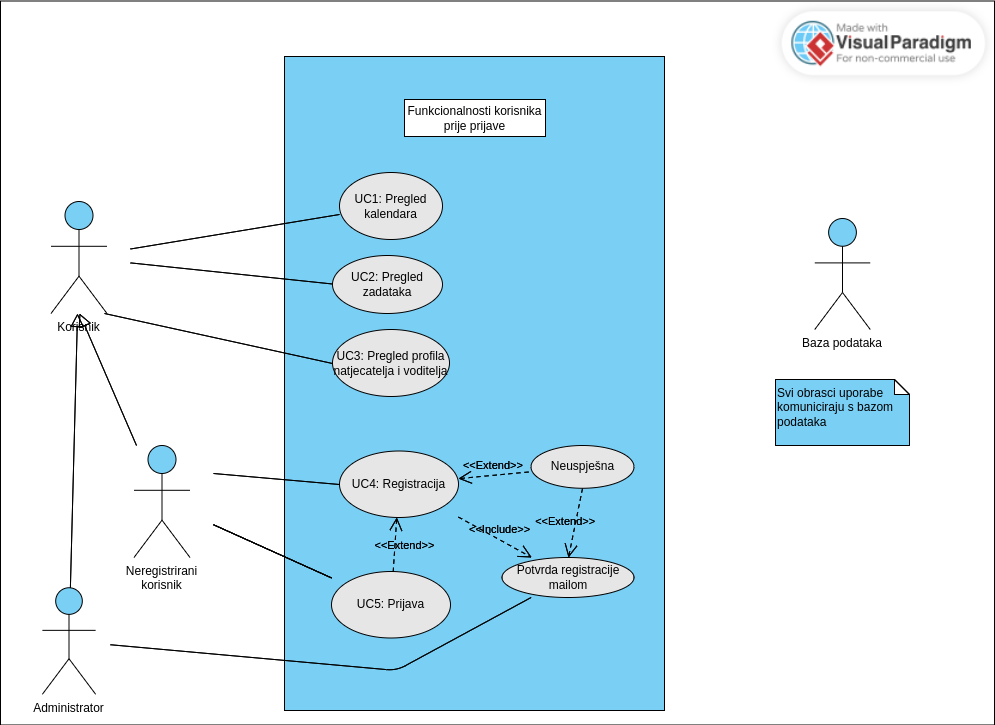
\includegraphics[scale=0.4]{dijagrami/obrasci_uporabe1.png} 
						\centering
						\caption{Obrasci uporabe - funkcionalnosti za neprijavljene korisnike}
						\label{fig:obrasci_uporabe1}
					\end{figure}
					
					\begin{figure}[H]
						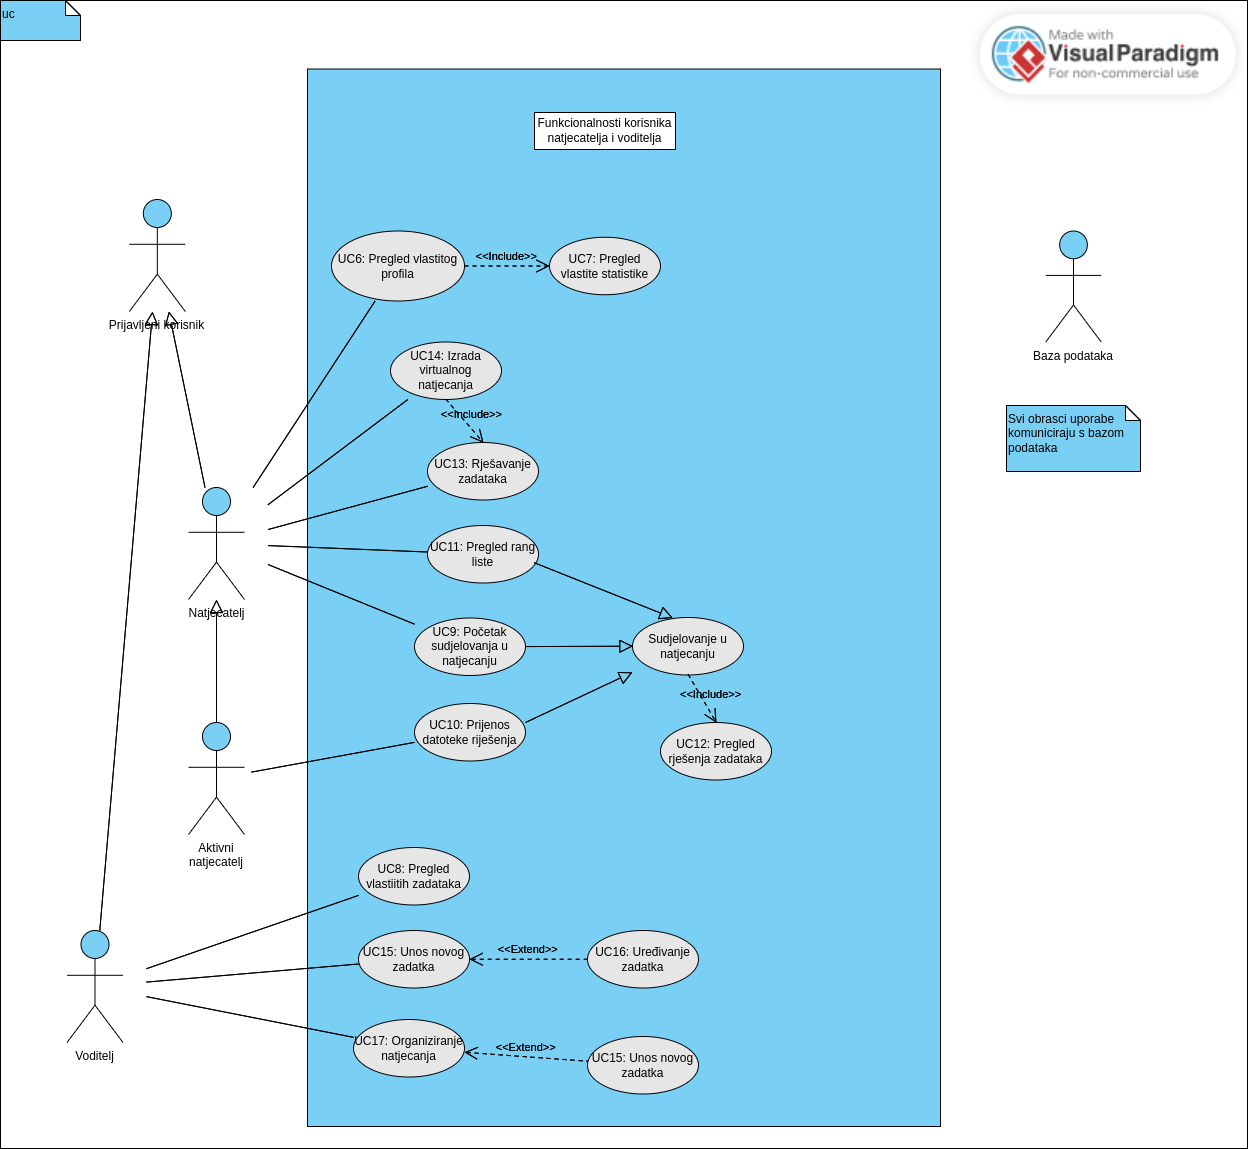
\includegraphics[scale=0.4]{dijagrami/obrasci_uporabe2.png} 
						\centering
						\caption{Obrasci uporabe - funkcionalnosti za natjecatelje i voditelje}
						\label{fig:obrasci_uporabe2}
					\end{figure}
					
					\begin{figure}[H]
						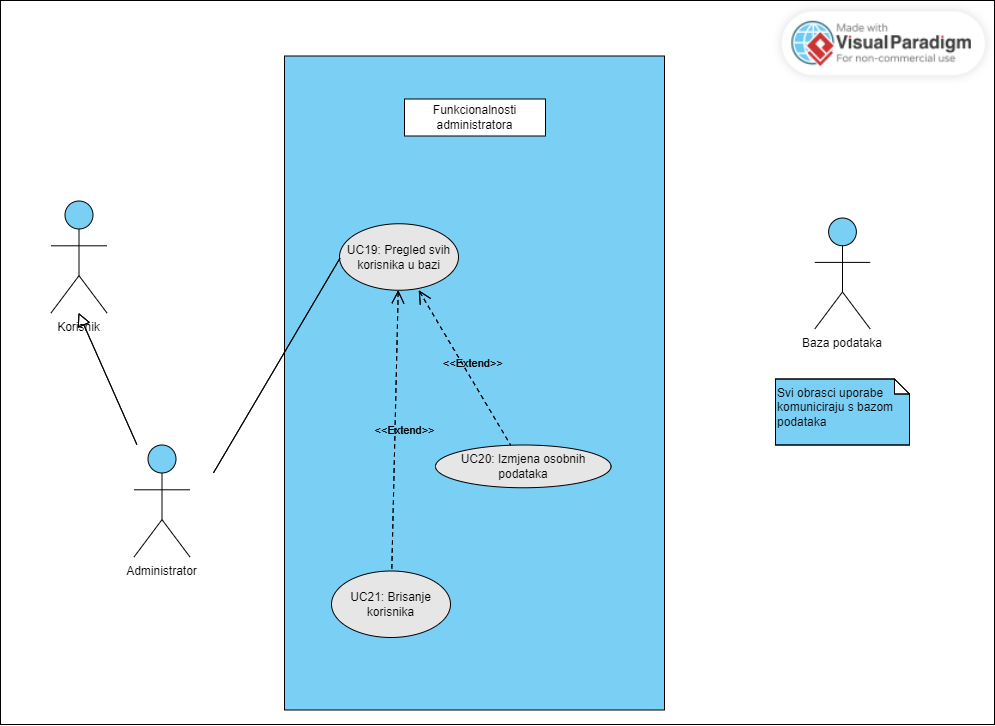
\includegraphics[scale=0.4]{dijagrami/obrasci_uporabe3.png} 
						\centering
						\caption{Obrasci uporabe - funkcionalnosti za administratore}
						\label{fig:obrasci_uporabe3}
					\end{figure}
				\eject		
				
			\subsection{Sekvencijski dijagrami}
				
%				\textbf{\textit{dio 1. revizije}}\\
%				
%				\textit{Nacrtati sekvencijske dijagrame koji modeliraju najvažnije dijelove sustava (max. 4 dijagrama). Ukoliko postoji nedoumica oko odabira, razjasniti s asistentom. Uz svaki dijagram napisati detaljni opis dijagrama.}


				\noindent \textbf{UC15 – unos novog zadatka}\\
				
				\noindent Korisnik prijavljen u sustav kao voditelj odabire opciju za stvaranje novog zadatka. Poslužitelj prikazuje formu s praznim poljima koje voditelj treba ispuniti podacima o zadatku. Točnije, potrebno je navesti naziv zadatka, broj bodova koje nosi, vremensko ograničenje izvršavanja, tekst zadatka i primjere za evaluaciju, a moguće je i odabrati opciju da zadatak bude stvoren kao privatan. Voditelj upisuje navedene podatke te ih šalje poslužitelju koji prvo provjerava da su svi podaci ispravno uneseni te da nema polja koja su ostala prazna. U slučaju neispravnosti podataka, poslužitelj prikazuje relevantnu poruku o problemu i ponovno omogućuje ispunjavanje forme. Nakon uspješne provjere, podaci se šalju bazi podataka koja ih sprema i time stvara novi zadatak. Ako sve prođe bez problema, baza podataka šalje potvrdu poslužitelju o uspješnom stvaranju novog zadatka, a poslužitelj zatim javlja korisniku da je njegov zahtjev uspješno proveden.
				
				\begin{figure}[H]
					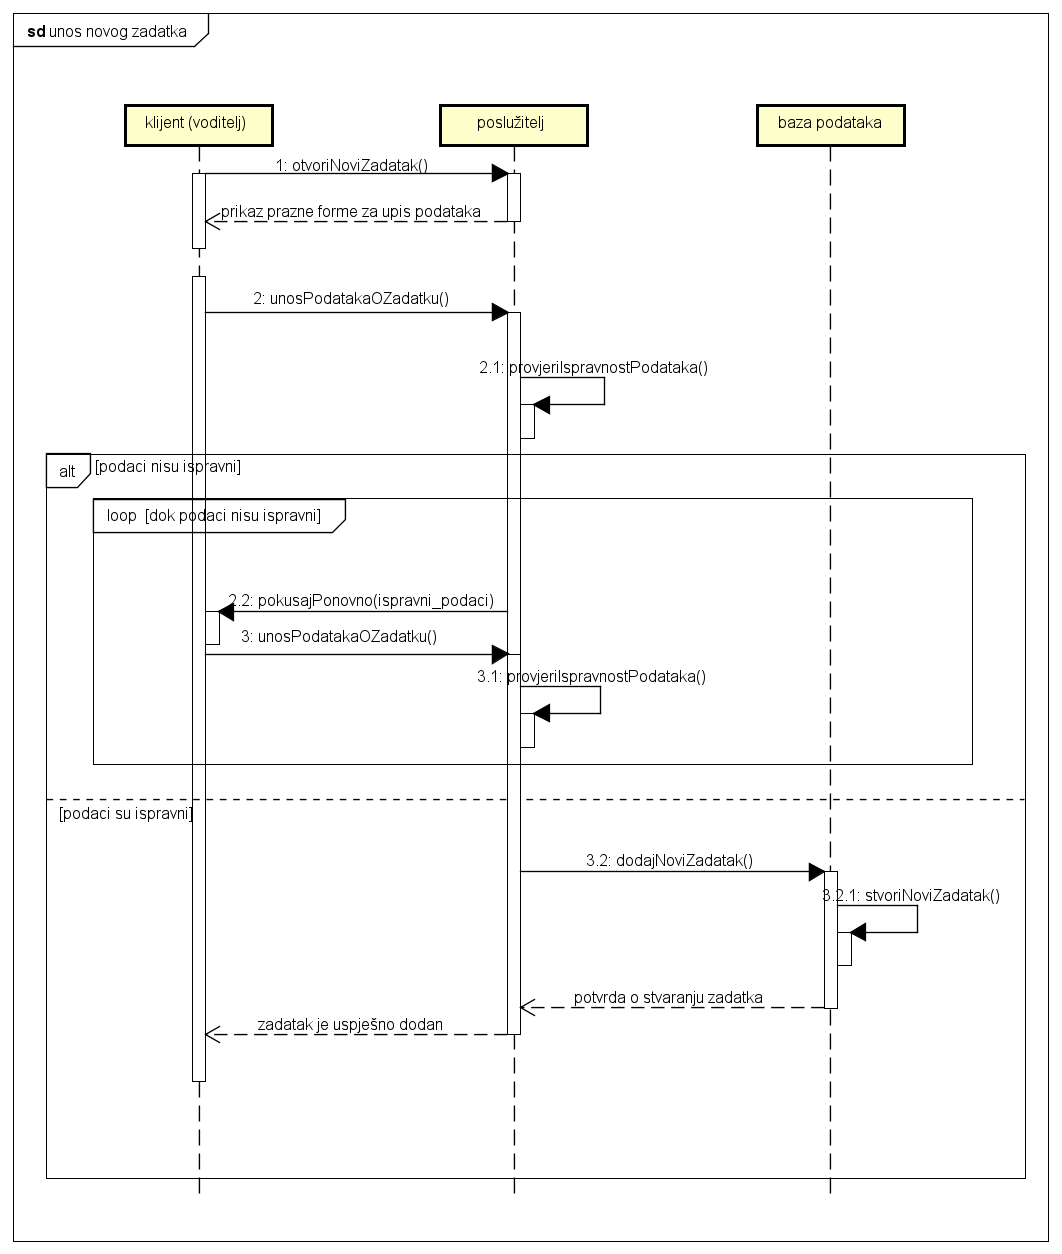
\includegraphics[scale=0.6]{dijagrami/sd15.png} 
					\centering
					\caption{Sekvencijski dijagram za obrazac uporabe - unos novog zadatka}
					\label{fig:sekvencijski1}
				\end{figure}
				\pagebreak
				
				\noindent \textbf{UC17 – organiziranje novog natjecanja}\\
				
				\noindent Korisnik prijavljen u sustav kao voditelj odabire opciju za stvaranjem novog natjecanja. Poslužitelj prikazuje formu s praznim poljima koje je voditelj dužan ispuniti informacijama o natjecanju. Potrebno je unijeti vrijeme početka i završetka natjecanja, broj zadataka, odabrati zadatke koji će biti aktivni te po želji učitati sličicu pehara kojom se nagrađuju najbolji natjecatelji. Nakon što voditelj upiše podatke i preda ih poslužitelju na obradu, poslužitelj će prvo provjeriti ispravnost dobivenih vrijednosti. U slučaju da je voditelj izostavio nešto i ostavio polje praznim, sustav će ga obavijestiti i zatražiti ponovni unos podataka. Nakon uspješno ispunjene forme i uspješno primljenih podataka, poslužitelj će ih proslijediti bazi podataka i zatražiti stvaranje novog natjecanja. Nakon pohrane, ako sve prođe bez problema, baza podataka bi trebala poslati povratnu informaciju poslužitelju o uspješnom stvaranju novog natjecanja, a poslužitelj bi zatim trebao javiti korisniku da je njegov zahtjev uspješno proveden.
				
				\begin{figure}[H]
					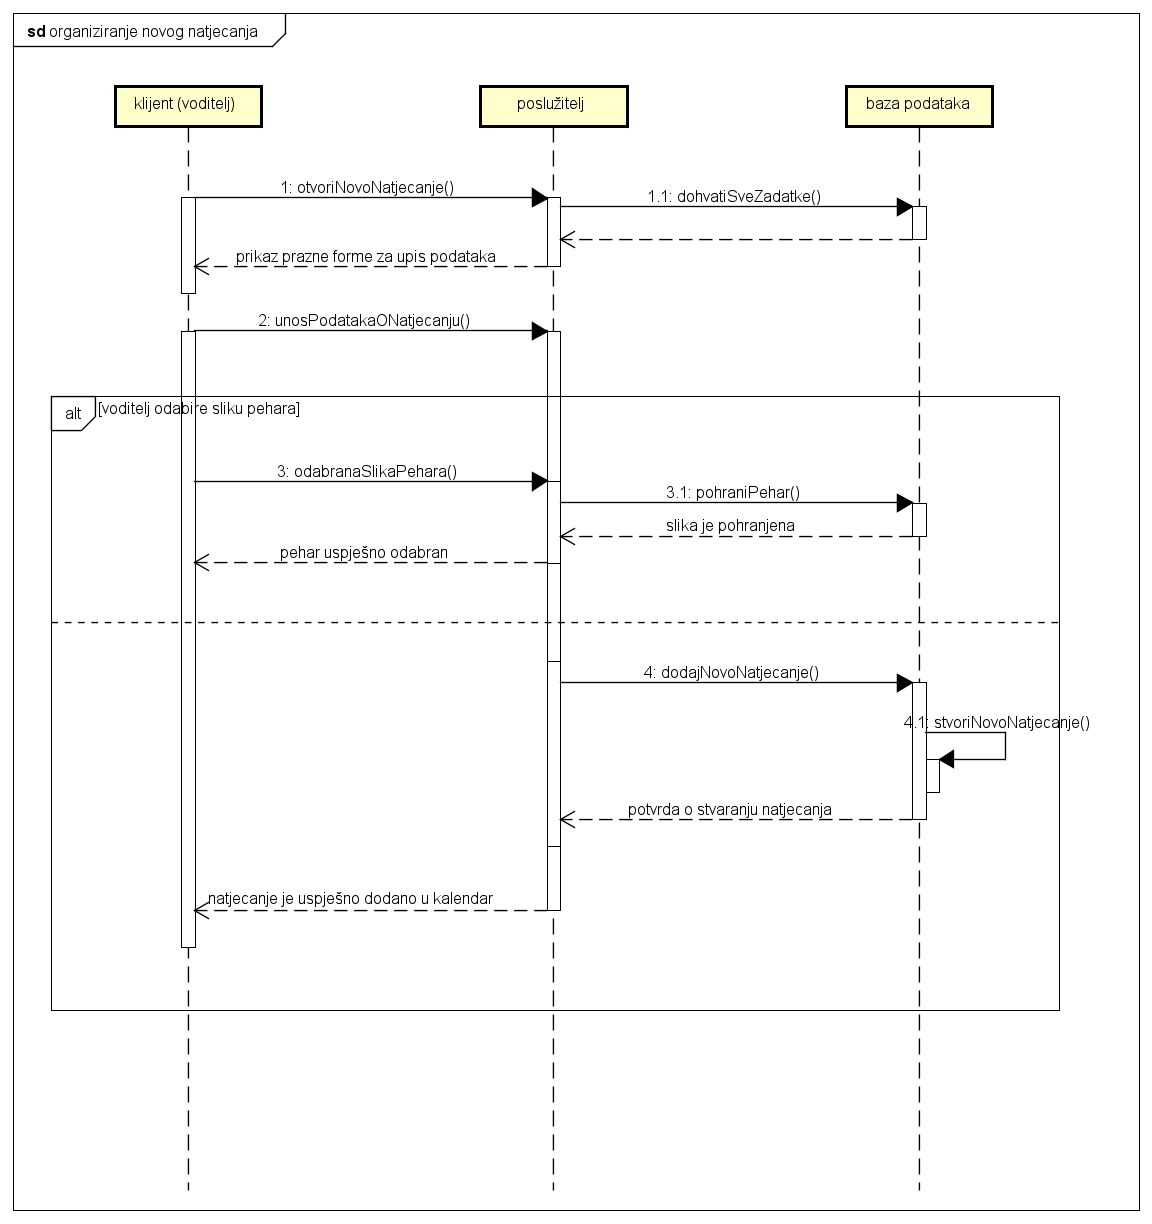
\includegraphics[scale=0.5]{dijagrami/sd17.png} 
					\centering
					\caption{Sekvencijski dijagram za obrazac uporabe - organiziranje novog natjecanja}
					\label{fig:sekvencijski2} 
				\end{figure}
				\pagebreak
				
				\noindent \textbf{UC10 i UC13 – rješavanje zadataka i prijenos datoteke}\\
				
				\noindent Korisnik prijavljen u sustav kao natjecatelj odabire opciju za prikaz svih objavljenih zadataka. Poslužitelj prikazuje popis svih javnih zadataka. Natjecatelj zatim bira zadatak koji želi pokušati riješiti pri čemu se otvara sučelje s tekstom zadatka i opcijom za prijenos datoteke rješenja. Natjecatelj odabire datoteku koju želi prenijeti kao rješenje i potvrđuje svoj odabir, a poslužitelj prosljeđuje datoteku do baze podataka koja ju sprema za prikaz prilikom nekih drugih funkcionalnosti. Na klijentov zahtjev predana datoteka se predaje evaluatoru koji pomoću definiranih primjera ulaza i izlaza određuje točnost rješenja zadatka i vraća ih poslužitelju. Poslužitelj sve rezultate sprema u bazu podataka i prikazuje klijentu u aplikaciji.
				
				\begin{figure}[H]
					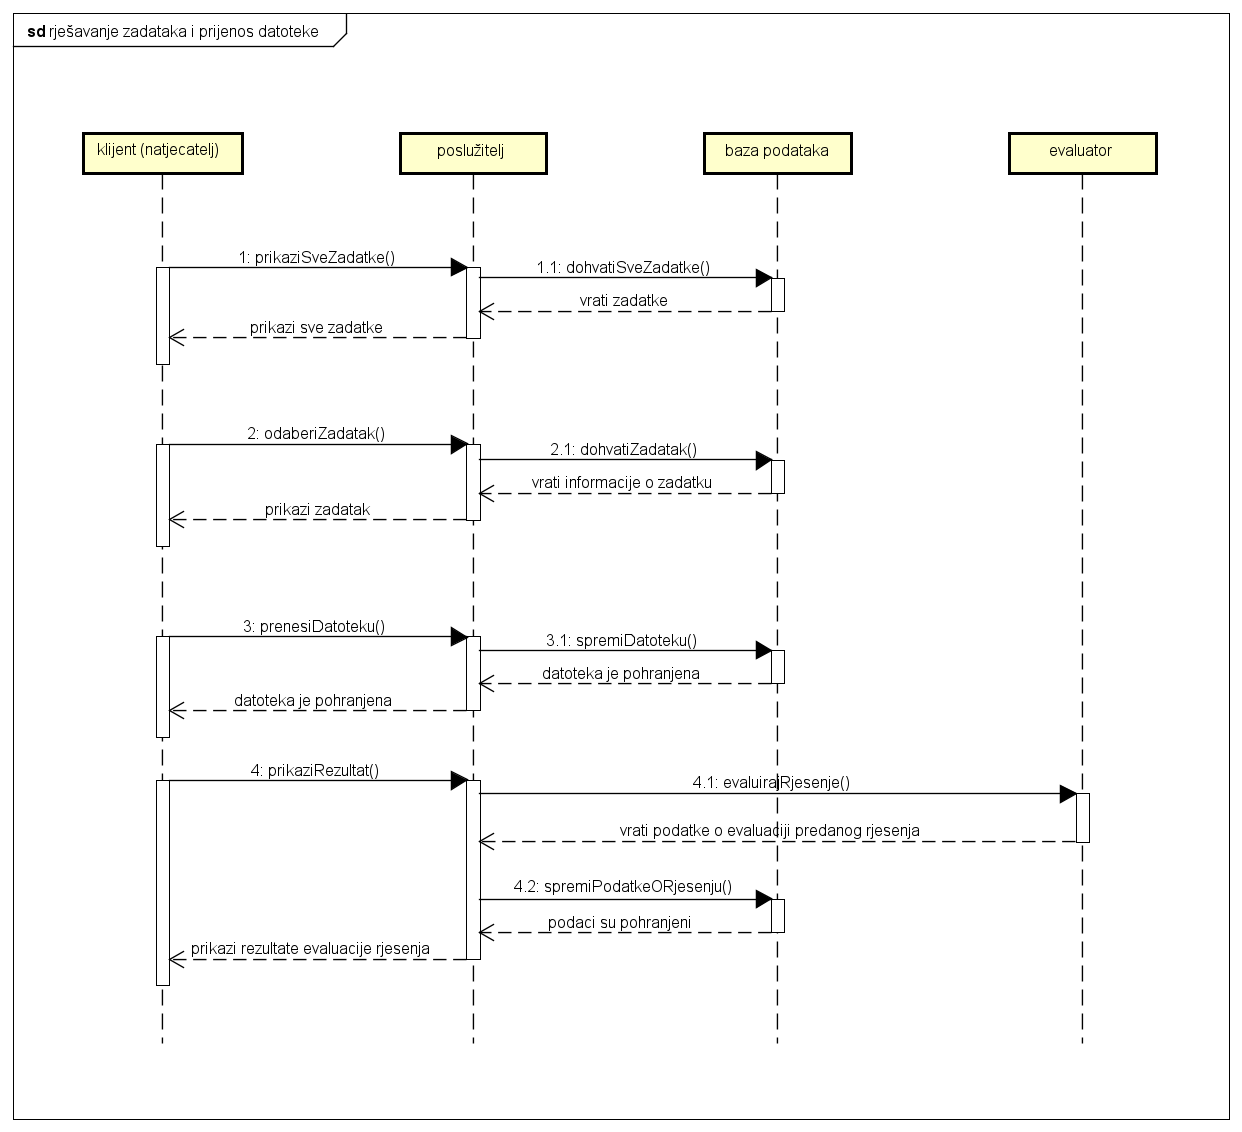
\includegraphics[scale=0.5]{dijagrami/sd10_sd13.png} 
					\centering
					\caption{Sekvencijski dijagram za obrasce uporabe -  rješavanje zadataka i prijenos datoteke}
					\label{fig:sekvencijski3}
				\end{figure}
				

				\eject	
		\section{Ostali zahtjevi}
			 
			 \begin{packed_item}
			 	
			 	\item Sustav treba dopustiti višekorisnički rad u stvarnom vremenu.
			 	\item Sustav treba biti jednostavan i intuitivan za korištenje tako da djeca nemaju problema sa razumijevanjem i snalaženjem na aplikaciji.
			 	\item Sustav se treba izgraditi kao mrežna aplikacija pomoću objektno-orijentiranih jezika.
			 	\item Sustav treba biti prilagođen za hrvatski jezik i abecedu prilikom prikaza i unosa tekstualnog sadržaja, uključujući i dijakritičke znakove.
			 	\item Pristup sustavu treba biti omogućen putem javne mreže.
			 	\item Sustav treba omogućiti evaluaciju rješenja zadataka za minimalno jedan programski jezik.
			 	\item Sustav treba biti takav da se sve funkcije izvršavaju brzo, ne duže od nekoliko sekundi, uključujući i evaluaciju rješenja zadataka.
			 	\item Baza podataka sustava mora biti kvalitetno i ispravno povezana sa sučeljem aplikacije.
			 	
			 \end{packed_item}
			 
	